\begin{figure*}[!t]

%%%
\begin{subfigure}{.482\textwidth}
%%%

    \resizebox{\linewidth}{!}{%

\begin{minipage}[t]{.625\linewidth}
    \centering
    \strut\vspace*{-9mm}\newline

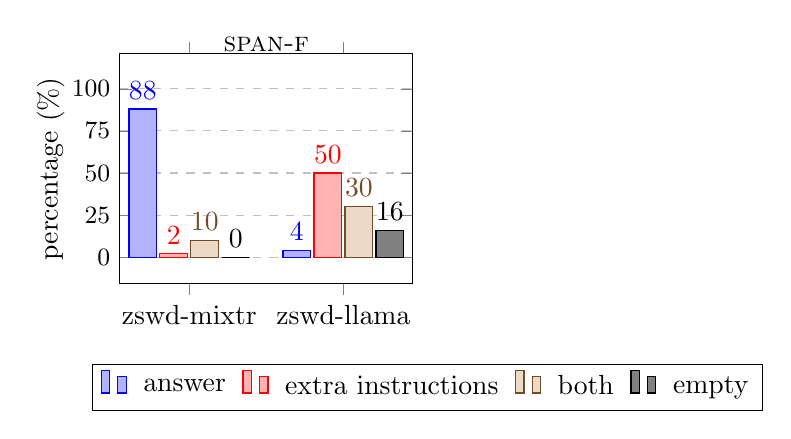
\begin{tikzpicture}
\begin{axis}[
    height=4.5cm,
    width=5.3cm,
    ymin=0, ymax=105,
    ybar=1.2pt,
    enlargelimits=0.15,
    enlarge x limits=0.45,
    legend style={at={(1.05,-0.35)},
      anchor=north, legend columns=-1, column sep=4pt},
    ylabel={percentage (\%)},
    ylabel style={yshift=-1.5mm},
    symbolic x coords={zswd-mixtr,zswd-llama},
    xtick=data,
    nodes near coords,
    nodes near coords align={vertical},
    title style={yshift=-3mm},
    title={\textsc{span-f}},
    ytick={0,25,50,75,100},
    ymajorgrids=true,
    grid style=dashed,
    yticklabel style = {font=\small}
]

% fine-grained
% [color=blue,postaction={pattern=vertical lines}]
\addplot coordinates {(zswd-mixtr,88) (zswd-llama,4)};
\addplot coordinates {(zswd-mixtr,2) (zswd-llama,50)};
\addplot coordinates {(zswd-mixtr,10) (zswd-llama,30)};
\addplot coordinates {(zswd-mixtr,0) (zswd-llama,16)};
\legend{answer, extra instructions, both, empty}
\end{axis}
\end{tikzpicture}

\end{minipage}\hfill
    \begin{minipage}[t]{.625\linewidth}
    \centering
    \strut\vspace*{-9mm}\newline

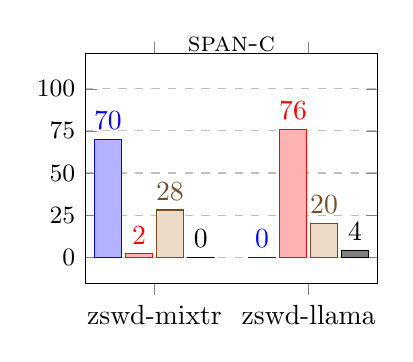
\begin{tikzpicture}
\begin{axis}[
    height=4.5cm,
    width=5.3cm,
    ymin=0, ymax=105,
    ybar=1.2pt,
    enlargelimits=0.15,
    enlarge x limits=0.45,
    legend style={at={(0.5,-0.35)},
      anchor=north, legend columns=-1, column sep=4pt},
    %ylabel={percentage (\%)},
    symbolic x coords={zswd-mixtr,zswd-llama},
    xtick=data,
    nodes near coords,
    nodes near coords align={vertical},
    title style={yshift=-3mm},
    title={\textsc{span-c}},
    ytick={0,25,50,75,100},
    ymajorgrids=true,
    grid style=dashed,
    legend style={draw=none},
    yticklabel style = {font=\small},
]

% coarse-grained
\addplot coordinates {(zswd-mixtr,70) (zswd-llama,0)};
\addplot coordinates {(zswd-mixtr,2) (zswd-llama,76)};
\addplot coordinates {(zswd-mixtr,28) (zswd-llama,20)};
\addplot coordinates {(zswd-mixtr,0) (zswd-llama,4)};
\legend{}
\end{axis}
\end{tikzpicture}

\end{minipage}


}%
	\caption{Analysis of the answers for \textsc{span} tasks.}
	\label{fig:generation-analysis-1}

%%%
\end{subfigure}%
\hfill
\begin{subfigure}{.482\textwidth}
%%%

    \resizebox{\linewidth}{!}{%

\begin{minipage}[t]{.625\linewidth}
    \centering
    \strut\vspace*{-9mm}\newline

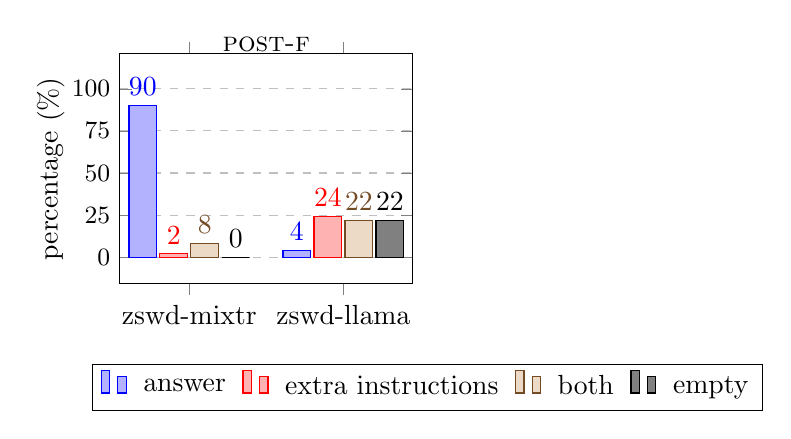
\begin{tikzpicture}
\begin{axis}[
    height=4.5cm,
    width=5.3cm,
    ymin=0, ymax=105,
    ybar=1.2pt,
    enlargelimits=0.15,
    enlarge x limits=0.45,
    legend style={at={(1.05,-0.35)},
      anchor=north, legend columns=-1, column sep=4pt},
    ylabel={percentage (\%)},
    ylabel style={yshift=-1.5mm},
    symbolic x coords={zswd-mixtr,zswd-llama},
    xtick=data,
    nodes near coords,
    nodes near coords align={vertical},
    title style={yshift=-3mm},
    title={\textsc{post-f}},
    ytick={0,25,50,75,100},
    ymajorgrids=true,
    grid style=dashed,
    yticklabel style = {font=\small}
]

% fine-grained
\addplot coordinates {(zswd-mixtr,90) (zswd-llama,4)};
\addplot coordinates {(zswd-mixtr,2) (zswd-llama,24)};
\addplot coordinates {(zswd-mixtr,8) (zswd-llama,22)};
\addplot coordinates {(zswd-mixtr,0) (zswd-llama,22)};
\legend{answer, extra instructions, both, empty}
\end{axis}
\end{tikzpicture}

\end{minipage}\hfill
    \begin{minipage}[t]{.625\linewidth}
    \centering
    \strut\vspace*{-9mm}\newline

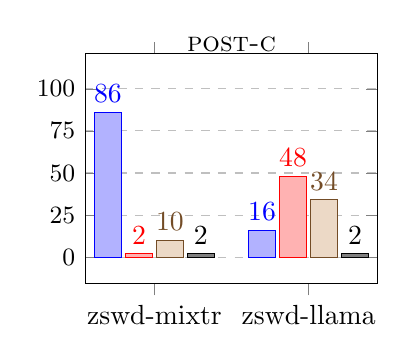
\begin{tikzpicture}
\begin{axis}[
    height=4.5cm,
    width=5.3cm,
    ymin=0, ymax=105,
    ybar=1.2pt,
    enlargelimits=0.15,
    enlarge x limits=0.45,
    legend style={at={(0.5,-0.35)},
      anchor=north, legend columns=-1, column sep=4pt},
    %ylabel={percentage (\%)},
    symbolic x coords={zswd-mixtr,zswd-llama},
    xtick=data,
    nodes near coords,
    nodes near coords align={vertical},
    title style={yshift=-3mm},
    title={\textsc{post-c}},
    ytick={0,25,50,75,100},
    ymajorgrids=true,
    grid style=dashed,
    legend style={draw=none},
    yticklabel style = {font=\small}
]

% coarse-grained
\addplot coordinates {(zswd-mixtr,86) (zswd-llama,16)};
\addplot coordinates {(zswd-mixtr,2) (zswd-llama,48)};
\addplot coordinates {(zswd-mixtr,10) (zswd-llama,34)};
\addplot coordinates {(zswd-mixtr,2) (zswd-llama,2)};
\legend{}
\end{axis}
\end{tikzpicture}

\end{minipage}


}%
	\caption{Analysis of the answers for \textsc{post} tasks.}
	\label{fig:generation-analysis-3}

%%%
\end{subfigure}%
%%%

\caption{Analysis of the \textbf{raw outputs} generated by LLMs across the four tasks according to whether they contain an actual \emph{answer}, \emph{extra instructions}, \emph{both} an actual answer and extra instructions, or an \emph{empty} response.}
\label{fig:analysis-general}

\end{figure*}